
\appendix



\begin{figure}
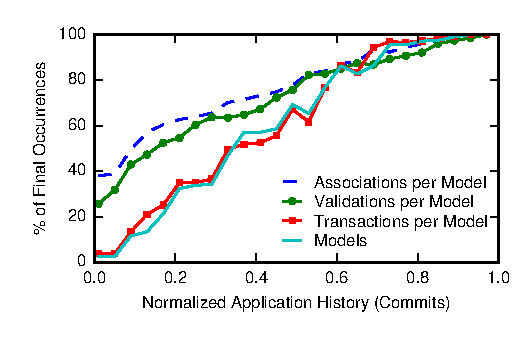
\includegraphics[width=\columnwidth]{figs/historical-median.pdf}\vspace{-2em}
\caption{Median use of Rails mechanisms over time.}
\label{fig:historical}
\end{figure}


\begin{figure}
  \newcommand{\skipht}{\\[-2em]}
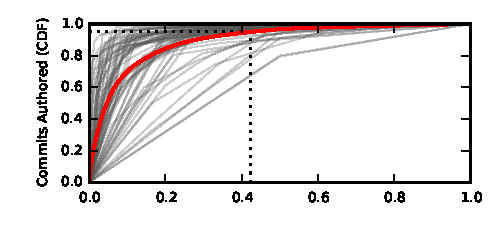
\includegraphics[width=\columnwidth]{figs/commit-authorship-cdf.pdf}\vspace{-2em}
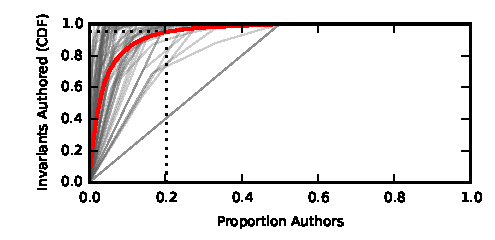
\includegraphics[width=\columnwidth]{figs/invariant-authorship-cdf.pdf}\vspace{-1em}
\caption{CDFs of authorship of invariants (validations plus
  associations) and commits. Bolded line
  shows the average CDF across projects, while faint lines show CDFs
  for individual projects. The dotted line shows the 95th percentile
  CDF value. }
\label{fig:cdfs}
\end{figure}

\begin{table*}
\scriptsize
\begin{tabular}{{|l}*{12}{l}{l|}}\hline
Name & Description & Authors & LoC Ruby & Commits &
 M & {\scriptsize T} & \scriptsize{PL} & \scriptsize{OL} & \scriptsize{V} &
 \scriptsize{A} & \scriptsize{Stars} &  \tiny{Githash} & \tiny{Last
   commit}\\\hline

Canvas LMS & {\scriptsize{Education}} & 132 & 308,113 & 12,889 & 161 & 46 & 12 & 1 & 354 & 839 & 1,251 & {\tiny\texttt{3fb8e69}} & {\tiny{10/16/14}}\\
OpenCongress & {\scriptsize{Congress data}} & 15 & 30,040 & 1,884 & 106 & 1 & 0 & 0 & 48 & 357 & 124 & {\tiny\texttt{850b602}} & {\tiny{02/11/13}}\\
Fedena & {\scriptsize{Education management}} & 4 & 48,359 & 1,471 & 104 & 5 & 0 & 0 & 153 & 317 & 262 & {\tiny\texttt{40cafe3}} & {\tiny{01/23/13}}\\
Discourse & {\scriptsize{Community discussion}} & 440 & 71,338 & 11,502 & 77 & 41 & 0 & 0 & 83 & 268 & 12,233 & {\tiny\texttt{1cf4a0d}} & {\tiny{10/20/14}}\\
Spree & {\scriptsize{eCommerce}} & 677 & 46,976 & 14,107 & 72 & 6 & 0 & 0 & 92 & 252 & 5,582 & {\tiny\texttt{aa34b3a}} & {\tiny{10/16/14}}\\
Sharetribe & {\scriptsize{Content management}} & 35 & 30,357 & 7,140 & 68 & 0 & 0 & 0 & 112 & 202 & 127 & {\tiny\texttt{8e0d382}} & {\tiny{10/21/14}}\\
ROR Ecommerce & {\scriptsize{eCommerce}} & 19 & 16,732 & 1,604 & 63 & 2 & 3 & 0 & 219 & 207 & 857 & {\tiny\texttt{c60a675}} & {\tiny{10/09/14}}\\
Diaspora & {\scriptsize{Social network}} & 388 & 31,361 & 14,640 & 63 & 2 & 0 & 0 & 66 & 128 & 9,571 & {\tiny\texttt{1913397}} & {\tiny{10/03/14}}\\
Redmine & {\scriptsize{Project management}} & 10 & 79,483 & 11,049 & 62 & 11 & 0 & 1 & 131 & 157 & 2,264 & {\tiny\texttt{e23d4d9}} & {\tiny{10/19/14}}\\
ChiliProject & {\scriptsize{Project management}} & 53 & 64,512 & 5,532 & 61 & 7 & 0 & 1 & 118 & 130 & 623 & {\tiny\texttt{984c9ff}} & {\tiny{08/13/13}}\\
Spot.us & {\scriptsize{Community reporting}} & 46 & 92,737 & 9,280 & 58 & 0 & 0 & 0 & 96 & 165 & 343 & {\tiny\texttt{61b65b6}} & {\tiny{12/02/13}}\\
Jobsworth & {\scriptsize{Project management}} & 46 & 24,469 & 7,890 & 55 & 10 & 0 & 0 & 86 & 225 & 478 & {\tiny\texttt{3a1f8e1}} & {\tiny{09/12/14}}\\
OpenProject & {\scriptsize{Project management}} & 63 & 82,764 & 11,185 & 49 & 8 & 1 & 3 & 136 & 227 & 371 & {\tiny\texttt{c1e66af}} & {\tiny{11/21/13}}\\
Danbooru & {\scriptsize{Image board}} & 25 & 27,812 & 3,738 & 47 & 9 & 0 & 0 & 71 & 114 & 238 & {\tiny\texttt{c082ed1}} & {\tiny{10/17/14}}\\
Salor Retail & {\scriptsize{Point of Sale}} & 26 & 18,007 & 2,259 & 44 & 0 & 0 & 0 & 81 & 309 & 24 & {\tiny\texttt{00e1839}} & {\tiny{10/07/14}}\\
Zena & {\scriptsize{Content management}} & 7 & 55,694 & 2,514 & 44 & 1 & 0 & 0 & 12 & 43 & 172 & {\tiny\texttt{79576ac}} & {\tiny{08/18/14}}\\
Skyline CMS & {\scriptsize{Content management}} & 7 & 10,241 & 894 & 40 & 5 & 0 & 0 & 28 & 89 & 127 & {\tiny\texttt{64b0932}} & {\tiny{12/09/13}}\\
Opal & {\scriptsize{Project management}} & 6 & 10,643 & 474 & 38 & 3 & 0 & 0 & 42 & 96 & 45 & {\tiny\texttt{11edf34}} & {\tiny{01/09/13}}\\
OneBody & {\scriptsize{Church portal}} & 33 & 19,867 & 3,976 & 36 & 3 & 0 & 0 & 97 & 140 & 1,041 & {\tiny\texttt{2dfbd4d}} & {\tiny{10/19/14}}\\
CommunityEngine & {\scriptsize{Social networking}} & 67 & 13,796 & 1,613 & 35 & 3 & 0 & 0 & 92 & 101 & 1,073 & {\tiny\texttt{a4d3ea2}} & {\tiny{10/16/14}}\\
Publify & {\scriptsize{Blogging}} & 93 & 16,555 & 5,067 & 35 & 7 & 0 & 0 & 33 & 50 & 1,274 & {\tiny\texttt{4acf86e}} & {\tiny{10/20/14}}\\
Comas & {\scriptsize{Conference management}} & 5 & 6,893 & 435 & 33 & 6 & 0 & 0 & 80 & 45 & 21 & {\tiny\texttt{81c25a4}} & {\tiny{09/09/14}}\\
BrowserCMS & {\scriptsize{Content management}} & 56 & 21,011 & 2,503 & 32 & 4 & 0 & 0 & 47 & 77 & 1,183 & {\tiny\texttt{d654557}} & {\tiny{09/30/14}}\\
RailsCollab & {\scriptsize{Project managment}} & 25 & 8,799 & 865 & 29 & 6 & 0 & 0 & 40 & 122 & 262 & {\tiny\texttt{9f6c8c1}} & {\tiny{02/16/12}}\\
Insoshi & {\scriptsize{Social network}} & 16 & 118,619 & 1,321 & 28 & 2 & 0 & 0 & 63 & 164 & 1,583 & {\tiny\texttt{9976cfe}} & {\tiny{02/24/10}}\\
OpenGovernment & {\scriptsize{Government data}} & 15 & 8,906 & 2,231 & 28 & 4 & 0 & 0 & 22 & 141 & 160 & {\tiny\texttt{fa80204}} & {\tiny{11/21/13}}\\
Tracks & {\scriptsize{Personal productivity}} & 89 & 17,312 & 3,121 & 27 & 2 & 0 & 0 & 24 & 43 & 639 & {\tiny\texttt{eb2650c}} & {\tiny{10/02/14}}\\
GitLab & {\scriptsize{Code management}} & 672 & 37,671 & 12,319 & 24 & 15 & 0 & 0 & 131 & 114 & 14,129 & {\tiny\texttt{72abe9f}} & {\tiny{10/20/14}}\\
Brevidy & {\scriptsize{Video sharing}} & 2 & 7,118 & 6 & 24 & 1 & 0 & 0 & 74 & 56 & 167 & {\tiny\texttt{d0ddb1a}} & {\tiny{01/18/14}}\\
Alchemy & {\scriptsize{Content management}} & 34 & 19,097 & 4,222 & 23 & 2 & 0 & 0 & 37 & 40 & 240 & {\tiny\texttt{91d9d08}} & {\tiny{10/20/14}}\\
Teambox & {\scriptsize{Project management}} & 48 & 32,252 & 3,155 & 22 & 2 & 0 & 0 & 56 & 116 & 1,864 & {\tiny\texttt{62a8b02}} & {\tiny{09/20/11}}\\
Fat Free CRM & {\scriptsize{Customer relationship}} & 99 & 20,754 & 4,144 & 21 & 3 & 0 & 0 & 39 & 92 & 2,384 & {\tiny\texttt{3dd2c62}} & {\tiny{10/17/14}}\\
linuxfr.org & {\scriptsize{FLOSS community}} & 29 & 8,060 & 2,271 & 20 & 1 & 0 & 0 & 50 & 50 & 86 & {\tiny\texttt{5d4d6df}} & {\tiny{10/14/14}}\\
Squash & {\scriptsize{Bug reporting}} & 28 & 15,663 & 231 & 19 & 6 & 0 & 0 & 87 & 62 & 879 & {\tiny\texttt{c217ac1}} & {\tiny{09/15/14}}\\
Shoppe & {\scriptsize{eCommerce}} & 14 & 3,115 & 349 & 19 & 1 & 0 & 0 & 58 & 34 & 208 & {\tiny\texttt{19e60c8}} & {\tiny{10/18/14}}\\
nimbleShop & {\scriptsize{eCommerce}} & 12 & 7,513 & 1,805 & 19 & 0 & 0 & 0 & 47 & 34 & 47 & {\tiny\texttt{4254806}} & {\tiny{02/18/13}}\\
Piggybak & {\scriptsize{eCommerce}} & 16 & 2,205 & 383 & 17 & 1 & 0 & 0 & 51 & 35 & 166 & {\tiny\texttt{2bed094}} & {\tiny{09/10/14}}\\
wallgig & {\scriptsize{Wallpaper sharing}} & 6 & 5,541 & 350 & 17 & 1 & 0 & 0 & 42 & 45 & 18 & {\tiny\texttt{4424d44}} & {\tiny{03/23/14}}\\
Rucksack & {\scriptsize{Collaboration}} & 7 & 5,309 & 445 & 17 & 3 & 0 & 0 & 18 & 79 & 169 & {\tiny\texttt{59703d3}} & {\tiny{10/05/13}}\\
Calagator & {\scriptsize{Online calendar}} & 48 & 8,877 & 1,766 & 16 & 0 & 0 & 0 & 8 & 11 & 196 & {\tiny\texttt{6e5df08}} & {\tiny{10/19/14}}\\
Amahi Platform & {\scriptsize{Home media sharing}} & 15 & 6,187 & 577 & 15 & 2 & 0 & 0 & 38 & 22 & 65 & {\tiny\texttt{5101c8b}} & {\tiny{08/20/14}}\\
Sprint & {\scriptsize{Project management}} & 5 & 3,053 & 71 & 14 & 0 & 0 & 0 & 50 & 45 & 247 & {\tiny\texttt{584d887}} & {\tiny{09/17/14}}\\
Citizenry & {\scriptsize{Community directory}} & 17 & 7,939 & 512 & 13 & 0 & 0 & 0 & 12 & 45 & 138 & {\tiny\texttt{e314fe4}} & {\tiny{04/01/14}}\\
Saasy & {\scriptsize{eCommerce}} & 2 & 161,092 & 21 & 12 & 5 & 0 & 0 & 41 & 117 & 520 & {\tiny\texttt{4fe610f}} & {\tiny{08/03/09}}\\
LovdByLess & {\scriptsize{Social network}} & 17 & 29,639 & 150 & 12 & 0 & 0 & 0 & 27 & 41 & 568 & {\tiny\texttt{26e79a7}} & {\tiny{10/09/09}}\\
lobste.rs & {\scriptsize{Link sharing}} & 24 & 4,927 & 624 & 12 & 8 & 0 & 0 & 20 & 40 & 646 & {\tiny\texttt{b0b9654}} & {\tiny{10/18/14}}\\
BucketWise & {\scriptsize{Personal finance}} & 10 & 4,343 & 258 & 12 & 2 & 0 & 0 & 11 & 46 & 484 & {\tiny\texttt{5c73f2b}} & {\tiny{06/10/12}}\\
Sugar & {\scriptsize{Forum}} & 13 & 7,590 & 1,316 & 11 & 1 & 0 & 0 & 20 & 53 & 89 & {\tiny\texttt{49ca79f}} & {\tiny{10/21/14}}\\
Comfy Mexican Sofa & {\scriptsize{Content management}} & 106 & 8,831 & 1,748 & 10 & 0 & 0 & 0 & 35 & 26 & 1,523 & {\tiny\texttt{fecef0c}} & {\tiny{10/09/14}}\\
Radiant & {\scriptsize{Content management}} & 100 & 15,124 & 2,385 & 9 & 3 & 0 & 1 & 26 & 12 & 1,554 & {\tiny\texttt{0c9ef9b}} & {\tiny{10/01/14}}\\
Refinery CMS & {\scriptsize{Content management}} & 438 & 10,797 & 9,112 & 9 & 0 & 0 & 0 & 16 & 8 & 2,979 & {\tiny\texttt{f4e24ef}} & {\tiny{10/20/14}}\\
Forem & {\scriptsize{Forum}} & 106 & 4,632 & 1,409 & 9 & 0 & 0 & 0 & 10 & 29 & 1,302 & {\tiny\texttt{519f2de}} & {\tiny{08/14/14}}\\
BostonRB & {\scriptsize{Ruby community}} & 40 & 2,128 & 889 & 7 & 0 & 0 & 0 & 18 & 12 & 199 & {\tiny\texttt{05fc100}} & {\tiny{10/21/14}}\\
Inkwell & {\scriptsize{Social networking}} & 6 & 6,731 & 156 & 7 & 0 & 0 & 0 & 4 & 51 & 327 & {\tiny\texttt{d1938d3}} & {\tiny{07/15/14}}\\
Boxroom & {\scriptsize{File sharing}} & 9 & 1,924 & 368 & 6 & 0 & 0 & 0 & 18 & 12 & 218 & {\tiny\texttt{1e74e06}} & {\tiny{10/18/14}}\\
Copycopter & {\scriptsize{Copy writing}} & 9 & 2,267 & 46 & 6 & 1 & 0 & 0 & 7 & 14 & 652 & {\tiny\texttt{d3607c4}} & {\tiny{06/28/12}}\\
Enki & {\scriptsize{Blogging}} & 29 & 4,584 & 562 & 6 & 1 & 0 & 0 & 5 & 7 & 835 & {\tiny\texttt{b793d48}} & {\tiny{12/01/13}}\\
Fulcrum & {\scriptsize{Project planning}} & 46 & 3,054 & 637 & 5 & 0 & 0 & 0 & 13 & 15 & 1,335 & {\tiny\texttt{8397de2}} & {\tiny{08/20/14}}\\
GitLab CI & {\scriptsize{Continuous integration}} & 80 & 3,650 & 870 & 5 & 2 & 0 & 0 & 11 & 13 & 1,188 & {\tiny\texttt{7d51134}} & {\tiny{10/17/14}}\\
Kandan & {\scriptsize{Persistent chat}} & 56 & 1,533 & 808 & 5 & 0 & 0 & 0 & 6 & 8 & 2,249 & {\tiny\texttt{15a8aab}} & {\tiny{10/06/14}}\\
Juvia & {\scriptsize{Commenting}} & 8 & 2,280 & 202 & 4 & 3 & 0 & 0 & 11 & 8 & 937 & {\tiny\texttt{43a1c48}} & {\tiny{05/09/14}}\\
Go vs Go & {\scriptsize{Go board game}} & 2 & 2,317 & 302 & 4 & 0 & 0 & 0 & 11 & 9 & 145 & {\tiny\texttt{c8d739d}} & {\tiny{02/21/13}}\\
Adopt-a-Hydrant & {\scriptsize{Civics}} & 14 & 14,163 & 1,242 & 3 & 0 & 0 & 0 & 11 & 8 & 182 & {\tiny\texttt{5b7ea0e}} & {\tiny{10/21/14}}\\
Selfstarter & {\scriptsize{Crowdfunding}} & 23 & 574 & 127 & 3 & 0 & 0 & 0 & 1 & 4 & 2,688 & {\tiny\texttt{740075f}} & {\tiny{05/16/14}}\\
Heaven & {\scriptsize{Code deployment}} & 19 & 2,083 & 387 & 2 & 0 & 0 & 0 & 2 & 2 & 163 & {\tiny\texttt{2d4162e}} & {\tiny{10/21/14}}\\
Carter & {\scriptsize{eCommerce}} & 3 & 1,052 & 70 & 2 & 1 & 0 & 0 & 0 & 12 & 22 & {\tiny\texttt{60ad49d}} & {\tiny{07/22/14}}\\
Obtvse & {\scriptsize{Blogging}} & 27 & 427 & 393 & 1 & 0 & 0 & 0 & 3 & 0 & 1,516 & {\tiny\texttt{1542856}} & {\tiny{03/21/13}}\\\hline
\textbf{Average:} &  & \textbf{69.21} & \textbf{26,380.48} & \textbf{2,953.31} & \textbf{29.21} & \textbf{3.87} & \textbf{0.24} & \textbf{0.10} & \textbf{53.00} & \textbf{96.04} & \textbf{1,272.42} &  & {\tiny\textbf{02/06/14}}\\

\hline
\end{tabular}
\caption{Corpus of applications used in analysis (M: Models, T:
  Transactions, PL: Pessimistic Locking, OL: Optimistic Locking, V:
  Validations, A: Associations). Stars record number of GitHub Stars
  as of October 2014.}
\label{table:app-summary}
\end{table*}

\small

\section{Analysis Methodology}

\label{sec:appendix-methodology}

To determine the occurrences and number of models, transactions, locks, validations, and associations in Rails, we used a very simple set of custom code analysis scripts. We do not consider the analysis techniques here a contribution; rather, our interest is in the output of the analysis.  (Though we hesitate to term this process ``program analysis,'' the scripts embody a very simple syntactic static analysis.) The syntactic approach proved portable between the many versions of Rails against which each application is linked; otherwise, porting between non-backwards-compatible Rails versions was difficult and, in fact, unsupported by several of the Rails code analysis tools we considered using as alternatives. The choice to use syntax as a means of distinguishing code constructs led to some ambiguity. To compensate, we introduced custom logic to handle esoteric syntaxes that arose in particular projects (e.g., some projects extend \texttt{ActiveRecord::Base} with a separate, project-specific base class, while some validation usages vary between constructs like \texttt{:validates\_presence} and \texttt{:validates\_presence\_of}).

To determine code authorship, we used the output of git \texttt{log} and \texttt{blame} and did not attempt any sophisticated entity resolution.

\section{Detailed Validation Behavior}

\subsection{Uniqueness Validation}
\label{sec:appendix-uniqueness-behavior}

When a controller attempts to \texttt{save} an ActiveRecord model instance $i$ of type $M$, if $M$ has a declared \texttt{:validates\_uniqueness} annotation on attribute $a$, the following steps will be performed during validation:

\begin{enumerate} 
\small

\item Assuming that instances of $M$ are stored in database table $T_M$ (with attribute $a$ stored in column $C_a$), Active Record will perform the equivalent of $$\texttt{SELECT 1 FROM $T_M$ where $C_a$ = $i.a$ LIMIT ONE;}$$ (\texttt{SELECT COUNT(*)} would be sufficient here as well, but this is not how the query is actually implemented).

\item If this result set is empty, the validation succeeds.

\item If this result set is not empty, the validation fails. If the validation was called during \texttt{save}, it returns \texttt{false}. If the validation was called during \texttt{save!}, it raises an \texttt{ActiveRecord::RecordInvalid} exception.

\end{enumerate}

This is a classic example of the phantom problem. As we mention in Section~\ref{sec:evaluation}, changing this \texttt{SELECT} call to \texttt{SELECT FOR UPDATE} would be sufficient (given an appropriate implementation of next-key locking). However, Rails is not implemented as such.

\subsection{Association Validation}
\label{sec:appendix-association-behavior}

 When a controller attempts to \texttt{save} an ActiveRecord model instance $i$ of type $M$, if $M$ has a declared \texttt{:belongs\_to} annotation on attribute $a$ pointing to attribute $b$ of model $N$ \textit{and} $M$ has a declared \texttt{:validates\_presence} annotation on attribute $a$, the following steps will be performed during validation:

\begin{enumerate} 
\small
\item Assuming that instances of $N$ are stored in database table $T_N$ (with attribute $b$ stored in column $C_b$), Active Record will perform the equivalent of $$\texttt{SELECT 1 FROM $T_N$ where $C_b$ = $i.a$ LIMIT ONE;}$$

\item If this result set is not empty, the validation succeeds.

\item If this result set is empty, the validation fails. If the validation was called during \texttt{save}, it returns \texttt{false}. If the validation was called during \texttt{save!}, it raises an \texttt{ActiveRecord::RecordInvalid} exception.

\end{enumerate}

\section{Experimental Description}
\label{sec:appendix-experiments}

\lstset{language=Ruby,basicstyle=\ttfamily\small,columns=fullflexible,frame=single}

We describe our applications from Section~\ref{sec:evaluation} in greater detail.

\subsection{Uniqueness Validation Schema}
\label{sec:appendix-uniqueness-schema}

We declare two models, each containing two attributes: \texttt{key}, a string, and \texttt{value}, also a string. The generated schema for each of the models, which we call \texttt{SimpleKeyValue} and \texttt{ValidatedKeyValue}, is the same. The schema for \texttt{SimpleKeyValue} is as follows:\vspace{-.5em}
\begin{lstlisting}
  create_table "validated_key_values", force: true do |t|
    t.string   "key"
    t.string   "value"
    t.datetime "created_at"
    t.datetime "updated_at"
  end
\end{lstlisting}\vspace{-.5em}
For the non-uniqueness-validated model, we simply require that the \texttt{key} and \texttt{value} fields are not null via a \texttt{presence: true} annotation.  For the ferally validated model, we add an additional \texttt{uniqueness: true} validation to the \texttt{key} field in the Active Record model. The remainder of the application consists of a simple View and Controller logic to allow us to \texttt{POST}, \texttt{GET}, and \texttt{DELETE} each kind of model instance programatically via HTTP.



\begin{comment}

\begin{lstlisting}
class SimpleKeyValue < ActiveRecord::Base
  validates :key, presence: true
  validates :value, presence: true
end
\end{lstlisting}

\end{comment}


\begin{comment}

\begin{lstlisting}
class ValidatedKeyValue < ActiveRecord::Base
  validates :key, presence: true, uniqueness: true
  validates :value, presence: true
end
\end{lstlisting}

\end{comment}



\subsection{Uniqueness Stress Test}
\label{sec:appendix-uniqueness-stress}

For the uniqueness stress test (Figure~\ref{fig:pk-stress}), we repeatedly attempt to create duplicate records. We issue a set of 64 concurrent requests to create instances with the \texttt{key} field set to an increasing sequence number ($k$, below) and repeat 100 times. At the end of the run, we count the number of duplicate records in the table:\vspace{-1em}
\begin{algorithm}[H]
\begin{algorithmic}
\For{model $m \in \{\texttt{SimpleKeyValue}, \texttt{ValidatedKeyValue}\}$}
  \For{$k \gets 1$ to $100$}
    \ParFor{$1$ to $64$}
      \State via HTTP: create new $m$ with \texttt{key=$k$}
     \EndParFor
   \EndFor
   \State dups $\gets $execute(\texttt{SELECT key, COUNT(key)-1 FROM $T_M$}
   \State \hspace{6.5em}\texttt{GROUP BY key HAVING COUNT(key) > 1;})
\EndFor
\end{algorithmic}
\end{algorithm}\vspace{-1em}
Under correct validation, all but one of the creation requests per key should fail.

\subsection{Uniqueness Workload Test}
\label{sec:appendix-uniqueness-workload}

For the uniqueness workload test (Figure~\ref{fig:pk-workload}), a set of 64 workers sequentially issues a set of 100 operations each. Each operation attempts to create a new model instance with the \texttt{key} field set to a random item generated according to the distributions described in Section~\ref{sec:evaluation}:\vspace{-1em}
\begin{algorithm}[H]
\begin{algorithmic}
\For{model $m \in \{\texttt{SimpleKeyValue}, \texttt{ValidatedKeyValue}\}$}
  \ParFor{$1$ to $64$}
    \For{$1$ to $100$}
      \State $k \gets$ \textit{pick new key according to distribution}
      \State via HTTP: create new $m$ with \texttt{key=$k$}
     \EndFor
   \EndParFor
   \State dups $\gets $execute(\texttt{SELECT key, COUNT(key)-1 FROM $T_M$}
   \State \hspace{6.5em}\texttt{GROUP BY key HAVING COUNT(key) > 1;})
\EndFor
\end{algorithmic}
\end{algorithm}

\subsection{Association Validation Schema}
\label{sec:appendix-association-schema}

We declare two sets of models, each containing two models each: a \texttt{User} model and a \texttt{Departments} model. Each \texttt{User} has a(n implicit) \texttt{id} (as generated by Rails ActiveRecord) and an integer corresponding \texttt{department\_i}. Each \texttt{Department} has an \texttt{id}. Both models have a timestamp of the last updated and creation time, as is auto-generated by Rails. Aside from the table names, both schemas are equivalent. Below is the schema for the non-validated users and departments:\vspace{-.5em}
\begin{lstlisting}
create_table "simple_users", force: true do |t|
    t.integer  "simple_department_id"
    t.datetime "created_at"
    t.datetime "updated_at"
end

create_table "simple_departments", force: true do |t|
  t.datetime "created_at"
  t.datetime "updated_at"
end
\end{lstlisting}\vspace{-.5em}
The two pairs of models vary in their validations. One pair of models has no validations or associations. The other pair of models contain validations, including rules for cascading deletions. Specifically, we place an association \texttt{has\_many :users, :dependent => :destroy} on the department, and, on the user, an association \texttt{belongs\_to :department} and validation \texttt{validates :department, :presence => true} (note that we only delete from Departments in our workload, below). Thus, on deletion of a model of type \texttt{ValidatedDepartment}, ActiveRecord will attempt to call \texttt{destroy} on each matching \texttt{ValidatedUser}.

\begin{comment}
\begin{lstlisting}
class SimpleDepartment < ActiveRecord::Base
end

class SimpleUser < ActiveRecord::Base
end
\end{lstlisting}

\begin{lstlisting}
class ValidatedDepartment < ActiveRecord::Base
  has_many :validated_users, :dependent => :destroy
end

class ValidatedUser < ActiveRecord::Base
  belongs_to :validated_department 
  validates :validated_department, :presence => true
end
\end{lstlisting}
\end{comment} 


\subsection{Association Stress Test}
\label{sec:appendix-association-stress}

For the association stress test (Figure~\ref{fig:fk-stress}), we repeatedly attempt to create orphan users. We issue a set of 64 concurrent requests to create Users belonging to a particular department, while simultaneously deleting that department and repeat 100 times. At the end of the run, we count the number of users with a department that does not exist:\vspace{-.5em}
\begin{algorithm}[H]
\begin{algorithmic}

\For{model $m \in \{\texttt{Simple}, \texttt{Validated}\}$}
  \For{$i \gets 1$ to $100$}
    \State via HTTP: create $m$Department with \texttt{id=$i$}
  \EndFor
  \For{$i \gets 1$ to $100$}
    \ParFor{$w \in 1$ to $65$}
      \If {$w = 1$}
        \State via HTTP: delete $m$Department with \texttt{id=$i$}
      \Else
        \State via HTTP: create new $m$User \texttt{department\_id=$i$}
      \EndIf        
     \EndParFor
   \EndFor
   \State orphaned $\gets $execute(``\texttt{SELECT $m$\_department\_id,}
   \State \hspace{8.5em}\texttt{COUNT(*) FROM $m$\_users AS U}
   \State \hspace{8.5em}\texttt{LEFT OUTER JOIN}
   \State \hspace{8.5em}\texttt{$m$\_departments AS D}
   \State \hspace{8.5em}\texttt{ON U.$m$\_department\_id = D.id}
   \State \hspace{8.5em}\texttt{WHERE D.id IS NULL}
   \State \hspace{8.5em}\texttt{GROUP BY $m$\_department\_id}
   \State \hspace{8.5em}\texttt{HAVING COUNT(*) > 0;}'')
\EndFor
\end{algorithmic}
\end{algorithm}

\subsection{Association Workload Test}
\label{sec:appendix-association-workload}

For the association workload test (Figure~\ref{fig:fk-workload}), we begin by creating a variable number of departments (Figure~\ref{fig:fk-workload} x-axis; $D$). We next have 64 concurrent clients simultaneously attempt to create users belonging to a random department and delete random departments (in a 10:1 ratio of creations to deletions, for 100 operations each). We end by counting the number of orphaned users, as above. \vspace{-1em}
\begin{algorithm}[H]
\begin{algorithmic}
\For{model $m \in \{\texttt{Simple}, \texttt{Validated}\}$}
  \For{$d \gets 1$ to $D$}
    \State via HTTP: create $m$Department with \texttt{id=$i$}
  \EndFor
  \ParFor{$w \in 1$ to $64$}
      \State $d \gets uniformRandomInt([1, D])$
      \If {$uniformRandomDouble([0, 1]) < \frac{1}{11}$}
        \State via HTTP: delete $m$Department with \texttt{id=$d$}
      \Else
        \State via HTTP: create new $m$User \texttt{department\_id=$d$}
      \EndIf        
   \EndParFor
   \State orphaned $\gets $ as above, in stress test
\EndFor
\end{algorithmic}
\end{algorithm}
